% The document class supplies options to control rendering of some standard
% features in the result.  The goal is for uniform style, so some attention 
% to detail is *vital* with all fields.  Each field (i.e., text inside the
% curly braces below, so the MEng text inside {MEng} for instance) should 
% take into account the following:
%
% - author name       should be formatted as "FirstName LastName"
%   (not "Initial LastName" for example),
% - supervisor name   should be formatted as "Title FirstName LastName"
%   (where Title is "Dr." or "Prof." for example),
% - degree programme  should be "BSc", "MEng", "MSci", "MSc" or "PhD",
% - dissertation title should be correctly capitalised (plus you can have
%   an optional sub-title if appropriate, or leave this field blank),
% - dissertation type should be formatted as one of the following:
%   * for the MEng degree programme either "enterprise" or "research" to
%     reflect the stream,
%   * for the MSc  degree programme "$X/Y/Z$" for a project deemed to be
%     X%, Y% and Z% of type I, II and III.
% - year              should be formatted as a 4-digit year of submission
%   (so 2014 rather than the accademic year, say 2013/14 say).
%
% Note there is a *strict* requirement for the poster to be in portrait 
% format so that we display them on the poster boards available.

\documentclass[]{templates/poster}

\usepackage{pifont}
\usepackage{caption}
\usepackage{subcaption}
\usepackage{graphicx}
\usepackage{amsthm}
\usepackage{wrapfig}

\DeclareGraphicsExtensions{.pdf}

\postertitle{Quantum speedup of the Travelling Salesman Problem for bounded-degree graphs}
\posterauthors{Dominic J. Moylett\textsuperscript{1,2,3}, Noah Linden\textsuperscript{4} and Ashley Montanaro\textsuperscript{4}}
\posteraffils{\textsuperscript{1}Quantum Engineering Technology Labs, University of Bristol\\\textsuperscript{2}Quantum Engineering Centre for Doctoral Training, University of Bristol\\\textsuperscript{3}Heilbronn Institute for Mathematical Research, University of Bristol\\\textsuperscript{4}School of Mathematics, University of Bristol}

\begin{document}

% -----------------------------------------------------------------------------

\begin{frame}{} 

\begin{columns}[t]
  \begin{column}{0.900\linewidth}
  \begin{block}{\Large Introduction and Main Results}
  The Travelling Salesman Problem (TSP) is one of the oldest and most famous problems in graph theory. As an $NP$-hard problem, it is known that any classical algorithm for exactly solving the problem must take superpolynomial time, otherwise $P = NP$. But little research has been undertaken on determining whether or not quantum algorithms can outperform classical algorithms for this problem.
  
  We demonstrate quadratic speedups for solving the TSP when the degree of any vertex in the graph is at most $3$. This is through applying a quantum speedup for backtracking algorithms developed by Montanaro [Mon15] to a pair of algorithms by Xiao \& Nagamochi [XN16a] for solving the TSP when the maximum degree of any vertex in the graph is $3$ and $4$, respectively. We then demonstrate polynomial speedups for graphs of higher degrees. 
  
  See arXiv:1612.06203 for further information.
  \end{block}
  \end{column}
\end{columns}

\begin{columns}[t]
  \begin{column}{0.422\linewidth}
  \begin{block}{\Large 1. The Travelling Salesman Problem}
  Let $G = (V, E)$ be a graph with $n$ vertices $V$ and $m$ edges $E$. Associated with $G$ is a cost function $C \colon E \rightarrow \mathbb{Z}^+$. A cycle $H$ on $G$ is a {\em Hamiltonian cycle} if it visits every vertex in $G$ exactly once. The Travelling Salesman Problem is to return the minimum cost Hamiltonian cycle.
  
  \begin{center}
  \begin{figure}
  \begin{subfigure}[t]{0.3\linewidth}
  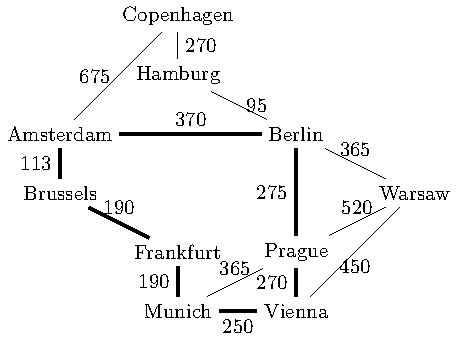
\includegraphics[width=\linewidth]{not_hamiltonian}
  \caption{\ding{55} Not a Hamiltonian cycle.}
  \end{subfigure}
  \begin{subfigure}[t]{0.3\linewidth}
  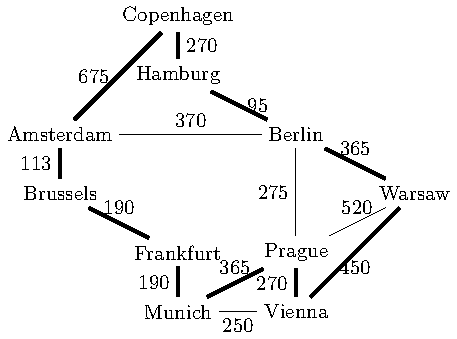
\includegraphics[width=\linewidth]{not_shortest}
  \caption{\ding{55} Not the shortest Hamiltonian cycle. (Length: $2983$ Minutes)}
  \end{subfigure}
  \begin{subfigure}[t]{0.3\linewidth}
  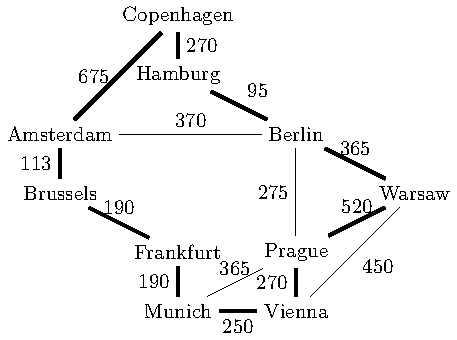
\includegraphics[width=\linewidth]{shortest}
  \caption{\ding{51} Solution to the Travelling Salesman Problem. (Length: $2938$ Minutes)}
  \end{subfigure}
  \end{figure}
  \end{center}
  \end{block}

  \begin{block}{\Large 2. Backtracking algorithms}
  Backtracking algorithms are algorithms used for solving Constraint Satisfaction Problems (CSPs), where the aim is to assign values to variables such that constraints are met. Backtracking algorithms take advantage of the CSP's local structure to solve the problem faster than na\"ive search. This is done using a predicate $P$, which checks if a partial assignment might satisfy the constraints, and a heuristic $h$, which recommends the next variable to assign.
  
  Montanaro [Mon15] demonstrated a quantum backtracking algorithm which showed a quadratic speedup in number of calls to $P$ and $h$ for the problem of finding a solution to a CSP.
  \end{block}
  \end{column}

  \begin{column}{0.422\linewidth}
  \begin{block}{\Large 3. The Xiao-Nagamochi algorithm for degree-3 graphs}
  Xiao-Nagamochi is a generalisation of Eppstein's algorithm [Epp07], described below:
  \begin{enumerate}
\item (Predicate) {\bf If} there aren't two distinct paths between any pair of vertices, then abort;
\item (Predicate \& Heuristic) {\bf Elseif} there is a vertex of degree 2, add both edges to $F$ and return $TSP3(G, F)$;
\item (Predicate \& Heuristic) {\bf Elseif} there is a vertex incident to two forced edges, remove any third edge and return $TSP3(G, F)$;
\item (Predicate \& Heuristic) {\bf Elseif} there is a pair of parallel edges and more than two vertices, remove the longer unforced edge and return $TSP3(G, F)$;
\item (Predicate \& Heuristic) {\bf Elseif} there is a triangle, reduce the triangle to a single vertex of degree 3 and return $TSP3(G, F)$;
\item (Predicate) {\bf Elseif} $G \setminus F$ is a disjoint collection of $4$-cycles, solve the problem directly via Lemma 3 of [Epp07] in polynomial time.
\item (Predicate \& Heuristic) {\bf Elseif} there is a cycle of 4 unforced edges incident to a forced edge, add the opposite edge to $F$ and return $TSP3(G, F)$;
\item (Heuristic) Pick an edge $e$ adjacent to an edge in $F$, call $TSP3(G\setminus \{e\}, F)$, $TSP3(G, F \cup \{e\})$ and return the shorter cycle;
\end{enumerate}

  By separating each step of the algorithm into predicate and heuristic as above, we can find a Hamiltonian cycle using [Mon15]. We repeat this process as a binary search $O(\log L)$ times to find the shortest Hamiltonian cycle, where $L = \max_{e \in E}(C(e))$.
  \end{block}
  \end{column}
\end{columns}
  
  \begin{columns}[t]
  \begin{column}{0.422\linewidth}

  \begin{block}{\Large 4. Expanding to higher-degree graphs}
  \begin{wrapfigure}[9]{r}{0.3\linewidth}
  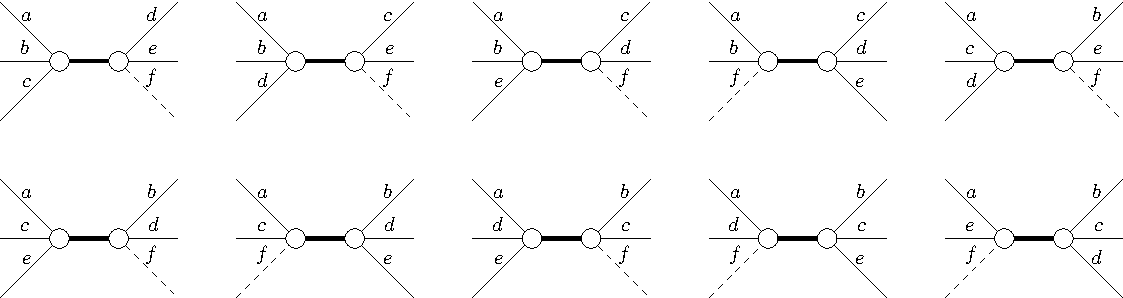
\includegraphics[width=\linewidth]{deg5}
  \caption{Example of splitting a vertex of degree 6 into two vertices of degree 4.}
  \end{wrapfigure}

  The same technique as in Sec.\ 3 produces a quadratic speedup for another algorithm for degree-4 graphs [XN16b]. Speedups for graphs of degrees 5 and 6 can be found by breaking vertices into two lower-degree vertices connected by a forced edge.
  
  Not all ways of splitting these vertices will preserve the shortest Hamiltonian cycle, but we can use D\"urr and H\o yer's minimum-finding algorithm [DH99] to search over all possible ways of splitting the vertices.
  \end{block}
  \end{column}

  \begin{column}{0.422\linewidth}
  \begin{block}{\Large References}
  [DH99] C. D\"urr and P. H\o yer, arXiv:quant-ph/9607014 (1999)

  \noindent[Epp07] D. Eppstein, Journal of Graph Algorithms and Applications, 11(1):61--81, (2007)

  \noindent[Mon15] A. Montanaro, arXiv:1509.02374 (2015)

  \noindent[XN16a] M. Xiao and H. Nagamochi, Algorithmica 74(2):713--741, (2016)

  \noindent[XN16b] M. Xiao and H. Nagamochi, Theory of Computing Systems, 58(2):241--272, (2016)
  \end{block}
  \end{column}
\end{columns}

\end{frame}

% -----------------------------------------------------------------------------

\end{document}



